\documentclass[border=10pt]{standalone}
\usepackage[svgnames]{xcolor}
\usepackage{amsmath}
\usepackage{pgfplots}
\pgfplotsset{compat=newest}
\usepackage[sfdefault]{FiraSans}
\usepackage{FiraMono}
\renewcommand*\familydefault{\sfdefault}
\begin{document}
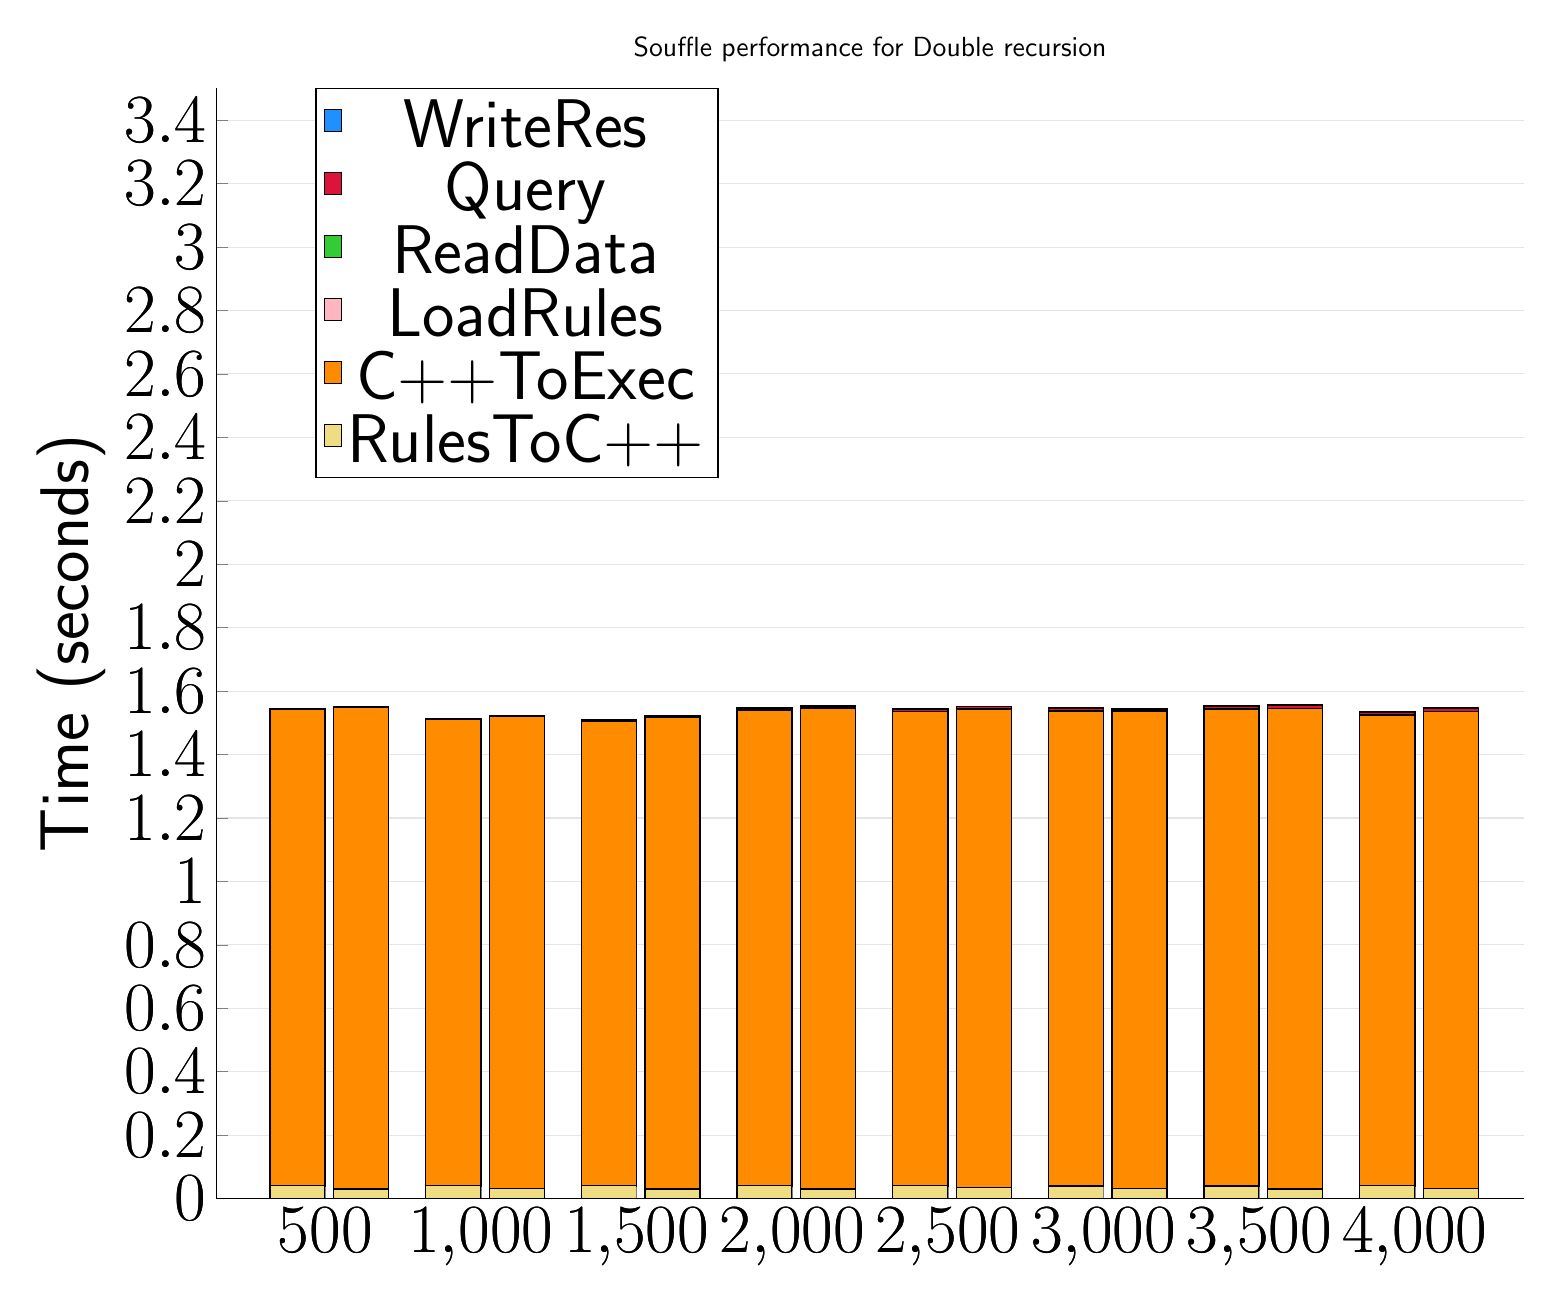
\begin{tikzpicture}
\begin{axis}[
   ybar stacked,
   title={Souffle performance for Double recursion},
   bar shift=-10pt,
   width=1.5\textwidth,
   bar width=0.7cm,
   ymajorgrids, tick align=inside,
   major grid style={draw=gray!20},
   xtick=data,
   ymin=0, ymax=3.5020000457763674,
   axis x line*=bottom,
   axis y line*=left,
   enlarge x limits=0.1,
   legend style={
       at={(0.23, 1)},
       anchor=north,
       legend columns=1,
       font=\Huge,
   },
   ylabel={Time (seconds)},
   label style={font=\Huge},
   tick label style={font=\Huge},
]
\addlegendimage{fill=DodgerBlue, draw=black, line width=0.2pt}
\addlegendentry{WriteRes}
\addlegendimage{fill=Crimson, draw=black, line width=0.2pt}
\addlegendentry{Query}
\addlegendimage{fill=LimeGreen, draw=black, line width=0.2pt}
\addlegendentry{ReadData}
\addlegendimage{fill=LightPink, draw=black, line width=0.2pt}
\addlegendentry{LoadRules}
\addlegendimage{fill=DarkOrange, draw=black, line width=0.2pt}
\addlegendentry{C++ToExec}
\addlegendimage{fill=LightGoldenrod, draw=black, line width=0.2pt}
\addlegendentry{RulesToC++}
\addplot +[fill=LightGoldenrod, draw=black, line width=0.5pt] coordinates {
    (500, 0.04100000858306885)
    (1000, 0.04100003242492676)
    (1500, 0.04100000858306885)
    (2000, 0.040999984741210936)
    (2500, 0.040999984741210936)
    (3000, 0.040000081062316895)
    (3500, 0.04000000953674317)
    (4000, 0.04100000858306885)
};
\addplot +[fill=DarkOrange, draw=black, line width=0.5pt] coordinates {
    (500, 1.5009999990463256)
    (1000, 1.4689999580383302)
    (1500, 1.462999987602234)
    (2000, 1.4990000009536744)
    (2500, 1.493999981880188)
    (3000, 1.496999979019165)
    (3500, 1.5020000457763671)
    (4000, 1.4829999923706054)
};
\addplot +[fill=LightPink, draw=black, line width=0.5pt] coordinates {
    (500, 0.00012037930000000001)
    (1000, 0.00012050000000000002)
    (1500, 0.00011224579999999998)
    (2000, 0.00011961260000000001)
    (2500, 0.00012351670000000002)
    (3000, 0.00011092089999999998)
    (3500, 0.00010602470000000001)
    (4000, 0.00010977090000000001)
};
\addplot +[fill=LimeGreen, draw=black, line width=0.5pt] coordinates {
    (500, 0.00038170820000000004)
    (1000, 0.0004842291)
    (1500, 0.0006147915999999999)
    (2000, 0.0006910665)
    (2500, 0.0007983709)
    (3000, 0.0009126331000000002)
    (3500, 0.0009516122000000002)
    (4000, 0.0010808152)
};
\addplot +[fill=Crimson, draw=black, line width=0.5pt] coordinates {
    (500, 0.0011507045)
    (1000, 0.002449495)
    (1500, 0.0037701870000000004)
    (2000, 0.004656138999999999)
    (2500, 0.005812282)
    (3000, 0.007076041999999999)
    (3500, 0.007908659)
    (4000, 0.009303318999999999)
};
\addplot +[fill=DodgerBlue, draw=black, line width=0.5pt] coordinates {
    (500, 0.0004972876)
    (1000, 0.0007937455000000002)
    (1500, 0.0009522207)
    (2000, 0.0011111620000000002)
    (2500, 0.0013662790000000002)
    (3000, 0.001559102)
    (3500, 0.001721354)
    (4000, 0.0019430450000000002)
};
\end{axis}
\begin{axis}[
   ybar stacked,
   bar shift=13pt,
   width=1.5\textwidth,
   bar width=0.7cm,
   ymajorgrids, tick align=inside,
   major grid style={draw=none},
   xtick=data,
   ymin=0, ymax=3.5020000457763674,
   axis x line*=none,
   axis y line*=none,
   enlarge x limits=0.1,
   label style={font=\Huge},
   tick label style={font=\Huge},
]
\addplot +[fill=LightGoldenrod, draw=black, line width=0.5pt] coordinates {
    (500, 0.030000000000000006)
    (1000, 0.031000000000000007)
    (1500, 0.030000000000000006)
    (2000, 0.030000000000000006)
    (2500, 0.033999999999999996)
    (3000, 0.031000000000000007)
    (3500, 0.030000000000000006)
    (4000, 0.031000000000000007)
};
\addplot +[fill=DarkOrange, draw=black, line width=0.5pt] coordinates {
    (500, 1.518)
    (1000, 1.489)
    (1500, 1.487)
    (2000, 1.516)
    (2500, 1.5099999999999998)
    (3000, 1.5050000000000001)
    (3500, 1.515)
    (4000, 1.504)
};
\addplot +[fill=LightPink, draw=black, line width=0.5pt] coordinates {
    (500, 0.00011949999999999999)
    (1000, 0.00011960000000000001)
    (1500, 0.00011150000000000001)
    (2000, 0.00011889999999999999)
    (2500, 0.00012269999999999997)
    (3000, 0.0001098)
    (3500, 0.00010529999999999998)
    (4000, 0.00010920000000000001)
};
\addplot +[fill=LimeGreen, draw=black, line width=0.5pt] coordinates {
    (500, 0.0003804999999999999)
    (1000, 0.00048340000000000004)
    (1500, 0.0006138999999999999)
    (2000, 0.0006900999999999999)
    (2500, 0.0007976999999999999)
    (3000, 0.000911)
    (3500, 0.0009507)
    (4000, 0.00108)
};
\addplot +[fill=Crimson, draw=black, line width=0.5pt] coordinates {
    (500, 0.0011500000000000002)
    (1000, 0.0024479000000000002)
    (1500, 0.0037695000000000007)
    (2000, 0.004655299999999999)
    (2500, 0.005810600000000001)
    (3000, 0.0070704)
    (3500, 0.007906199999999999)
    (4000, 0.009300300000000001)
};
\addplot +[fill=DodgerBlue, draw=black, line width=0.5pt] coordinates {
    (500, 0.00047829999999999997)
    (1000, 0.000695)
    (1500, 0.0009360999999999999)
    (2000, 0.0011103)
    (2500, 0.0013639999999999998)
    (3000, 0.0015537)
    (3500, 0.0016866000000000003)
    (4000, 0.0019223)
};
\end{axis}
\end{tikzpicture}

\end{document}
